\documentclass{beamer}
%
% Choose how your presentation looks.
%
% For more themes, color themes and font themes, see:
% http://deic.uab.es/~iblanes/beamer_gallery/index_by_theme.html
%
\mode<presentation>
{
  \usetheme{Madrid}      % or try Darmstadt, Madrid, Warsaw, ...
  \usecolortheme{beaver} % or try albatross, beaver, crane, ...
  \usefonttheme{serif}  % or try serif, structurebold, ...
  \setbeamertemplate{navigation symbols}{}
  \setbeamertemplate{caption}[numbered]
} 
\usepackage{graphicx}

\usepackage[english]{babel}
\usepackage[utf8x]{inputenc}
\usepackage{xcolor}
\usepackage{listings}
\lstset
{
    language=[LaTeX]TeX,
    breaklines=true,
    basicstyle=\tt\scriptsize,
    %commentstyle=\color{green}
    keywordstyle=\color{blue},
    %stringstyle=\color{black}
    identifierstyle=\color{magenta},
}

\title[Topics on Financial Markets]{Money in Search Equilibrium, in Competitive Equilibrium, and in Competitive Search Equilibrium}
\author{G. Rocheteau and R. Wright}
\date{Econometrica 2005}

%\AtBeginSection[]
%\{
  %\\begin{frame}<beamer>
    %\\frametitle{Outline}
    %\\tableofcontents[currentsection,currentsubsectio%\n]
  %\\end{frame}
%\}

\begin{document}

\begin{frame}
  \titlepage
\end{frame}

\begin{frame}<beamer>
\frametitle{Outline}
\tableofcontents
\end{frame}
  
\section{Introduction}

\begin{frame}{Introduction}
\begin{itemize}
    \item Until now, we discussed what frictions are essential for money.
    \begin{itemize}
        \item Kiyotaki and Wright [1993]: double coincidence problem
        \item Kocherlakota [1998]: imperfect memory/ record keeping technology
        \item Williamson and Sanches [2008]: limited commitment/ enforcement
    \end{itemize}
    \item However, we haven't analyzed the role of money and equilibrium under different market structures.
\end{itemize}
\end{frame}

\begin{frame}{Introduction}
\begin{itemize}
    \item Why the market structure matters?
    \begin{itemize}
        \item The pricing mechanism itself may cause the inefficiency of allocation. (e.g. bargaining in the random matching)
        \item The equilibrium and policy effects may depend on the the market structure.
    \end{itemize}
    \item Q: When the market structure changes, would our perceptions of money and policy implication remain robust?
\end{itemize}
\end{frame}

\begin{frame}{Introduction}
    \begin{itemize}
        \item This paper compares the efficiency of allocation and policies under three different pricing mechanisms/equilibrium concepts.
        \begin{itemize}
            \item bargaining (search equilibrium)
            \item Walrasian pricing (competitive equilibrium)
            \item pricing posting with directed search (competitive search equilibrium)
        \end{itemize}
    \end{itemize}
\end{frame}

\begin{frame}{Introduction}
    \begin{itemize}
        \item Based on Lagos and Wright [2002], this paper introduces two important settings into the model.
        \begin{itemize}
            \item Heterogeneous agents in the market
            \item Generalized matching technology and an entry decision by one side of the  market
        \end{itemize}
        \item This framework allows to apply the similar analysis as Moen [1997] in  monetary economies.
    \end{itemize}
\end{frame}

\begin{frame}{Introduction}
    \begin{itemize}
        \item The holdup problem and search externalities play critical roles in our analysis.
        \begin{itemize}
            \item the holdup problem: Agents have to carry the money from the last period. The cost of bringing money is inflation and the gain of it is the share of trade payoff.
            \item the search externalities
        \end{itemize}
        \item Under the competitive and competitive search equilibrium, the holdup problem can be eliminated; however, only at the  latter one, search externalities are internalized.
    \end{itemize}
\end{frame}
\section{Environment}

\begin{frame}{Environment}
    \begin{itemize}
        \item Time is discrete and continues forever. Each period is divided by two subperiods, day and night.
        \begin{itemize}
            \item Day: centralized and frictionless market 
            \item Night: depending on which pricing mechanism
        \end{itemize}
        \item There is a continuum of agents divided into two types, sellers and buyers.
        \begin{itemize}
            \item Sellers cannot consume during the night.
            \item Buyers cannot produce during the night.
        \end{itemize}
    \end{itemize}
\end{frame}

\begin{frame}{Environment}
    \begin{itemize}
        \item At the beginning of the day, sellers decide whether to join the market by entry condition.
        \item the measure of buyers: 1
        \item the measure of sellers: $n \geq 0$ 
        \begin{itemize}
            \item $\alpha(n)$: the probability each buyer gets an opportunity to trade
            \item $\alpha'(n) > 0$, $\alpha''(n) < 0$, $\alpha(n) \leq \min\{1,n\}$, $\alpha(0) = 0$, and $\alpha(\infty) = 1$
        \end{itemize}
        \item money: $M_{t}$ growing at the constant rate $\gamma_{t}$
    \end{itemize}
    
\end{frame}

\begin{frame}{Environment}
    \begin{itemize}
        \item $x,y$: the consumption and production during day, respectively
        \item $q$: the consumption and production during night
 
        \item A buyer's instantaneous utility function is represented by:
        \begin{align*}
         U^{b}(x,y,q) = \underbrace{v(x) - y}_{\text{day}}  + \underbrace{\beta_{d} u(q)}_{\text{night}}
        \end{align*}
        \item A seller's instantaneous utility function is represented by:
        \begin{align*}
         U^{s}(x,y,q) = \underbrace{v(x) - y}_{\text{day}}  - \underbrace{\beta_{d} c(q)}_{\text{night}}
        \end{align*}
        where $\beta_{d}$ is a discount factor between day and night and $v(\cdot)$, $ u(\cdot)$ and $c(\cdot)$ satisfy classical assumptions.

    \end{itemize}
    
\end{frame}
\section{Recursive Problems}
\begin{frame}{Bellman's Equations}
    \begin{itemize}
        \item Value Functions for agents in the night market can be shown as:
        \begin{align*}
            V^{b}(m_{b}) = \alpha(n)\left\{ u(q)+\beta_{n}W_{+1}^{b}(m_{b}-d)\right\} \\+\left[1-\alpha(n)\right]\beta_{n} W_{+1}^{b}(m_{b})\\
            V^{s}(m_{s}) = \frac{\alpha(n)}{n}\left\{ -c(q)+\beta_{n}W_{+1}^{s}(m_{s}+d)\right\} \\+\left[1-\frac{\alpha(n)}{n}\right]\beta_{n} W_{+1}^{s}(m_{s})-k
        \end{align*}
        where $\beta_{n}$ is a discount factor between night and day and night and $k$ is entry cost.
    \end{itemize}
    
\end{frame}

\begin{frame}{Bellman's Equations}
    \begin{itemize}
        \item The problems of agents in the day market are:
        \begin{align*}
            W^{i}(m_{i}) = \max_{\hat{m_{i}},x,y}\left\{v(x)-y+\beta_{d}V^{i}(\hat{m_{i}})\right\}\\
            \text{s.t. } 
            \begin{cases}\phi \hat{m_{i}} + x = \phi(m_{i}+T)+y & i = b\\ \phi \hat{m_{i}} + x = \phi m_{i} +y & i = s\end{cases}
        \end{align*}
        where $T$ is the lump-sum transfer employed by the government.
    \end{itemize}
    
\end{frame}
\begin{frame}{Bellman's Equations}
    \begin{itemize}
        \item F.O.C.
        \begin{align*}
            -\phi+\beta_{d}V_{m}^{i}(\hat{m_{i}}) \leq 0, = 0 \text{ if } \hat{m_{i}} > 0, i \in \{s,b\}
        \end{align*}
        \item The entry-free condition says $V^{s}(0) = 0$.
        \begin{align*}
            \frac{\alpha(n)}{n}\left[ -c(q)+\beta_{n}\phi_{+1}d\right]  =k
        \end{align*}
    \end{itemize}
\end{frame}

\begin{frame}{Bellman's Equations}
    \begin{itemize}
        \item There are some observations behind the equations.
        \begin{itemize}
            \item In the night market, no matter what the pricing mechanism we apply, the contract doesn't depend on the seller's money holding.
            \item The instantaneous utility functions in the day are quasi-linear, so there is no wealth effect on $m_{i}$.
            \item Given $\gamma \geq \beta = \beta_{d}\beta_{n}$, sellers wouldn't hold any money. Hence, $m_{s} = 0$ and $m_{b} = M$.
        \end{itemize}
    \end{itemize}
\end{frame}

\begin{frame}{Efficiency}
    \begin{itemize}
        \item A social planner chooses $(q,n,x_{s},x_{b})$ to maximize social welfare.
        \item Welfare: $\Omega = n(1-\beta)V^{s}(0)+(1-\beta)V^{b}(M)$
        \begin{align*}
            u'(q)-c'(q) = 0\\
            \alpha'(n)\left[u(q)-c(q)\right] = k\\
            v'(x_{i}) = 1, i\in \{s,b\}
        \end{align*}
        \item The efficiency consists of two parts: the number of trades, $n^{*}$ and the amount exchanged in each trade, $q^{*}$.
    \end{itemize}
    
\end{frame}

\section{Equilibrium}

\begin{frame}{Search Equilibrium}
    \begin{itemize}
        \item A buyer is matched with a seller randomly and they decide the contract $(q,d) $ by the Nash bargaining solution.  
        \item Given the bargaining power of a buyer $\theta \in [0,1]$, the problem is:
     \begin{align*}
         \max &\left[u(q)+\beta_{n}W_{+1}^{b}(m_{b}-d)-W_{+1}^{b}(m_{b})\right]^_{\theta}\\\times &\left[-c(q)+\beta_{n}W_{+1}^{s}(m_{s}+d)-W_{+1}^{s}(m_{s})\right]^_{1-\theta}\\
         &\text{s.t. } d\leq m_{b}
     \end{align*}
    \item Note: the linearity of $W(\cdot)$ 

    \end{itemize}
\end{frame}

\begin{frame}{Search Equilibrium}
    \begin{itemize}
        \item Given $\gamma \geq \beta$, $m_{b} < m^{*}$, where $m^{*}$ is the unbinding solution.
        \item F.O.C.
        \begin{align*}
            \beta_{n}\phi_{+1}m_{b} = \frac{\theta u'(q)c(q)+(1-\theta)c'(q)u(q)}{\theta u'(q)+(1-\theta)c'(q)} = g(q)
         \end{align*}
         \item Take the derivative of $V^{b}(m_{b})$ and combine it with the F.O.C
        \begin{align*}
            &V_{m}^{b}(m_{b})=\alpha(n)\left[u'(q)\frac{\partial q}{\partial m_{b}}-\beta_{n}\phi_{}\right]+\beta_{n}\phi_{+1} = \frac{\phi}{\beta_{d}}\\
            &\Rightarrow \frac{\gamma-\beta}{\beta\alpha(n)}+1 = \frac{u'(q)}{g'(q)}
        \end{align*}
        \item Free entry condition
        \begin{align*}
            \frac{\alpha(n)}{n}\frac{(1-\theta)c'(q)}{\theta u'(q)+(1-\theta)c'(q)}\left[u(q)-c(q)\right] = k
        \end{align*}

        
    \end{itemize}
\end{frame}

\begin{frame}{Search Equilibrium}
    \begin{itemize}
    \item Given the following assumptions, we can promise the existence of the solution  $(q,m_{b},d)\in \mathbb{R}^{3}_{+}$ satisfying the above three equations.
    \begin{itemize}
        \item $\lim_{q\rightarrow0}u'(q)/g'(q) =\infty$ and $u'(q)/g'(q)$ is strictly decreasing, $ \forall q<q^{*}$
        \item $\exists q $ s.t. $k<            \frac{\alpha(n)}{n}\frac{(1-\theta)c'(q)}{\theta u'(q)+(1-\theta)c'(q)}\left[u(q)-c(q)\right]$
    \end{itemize}
        \item Since $\theta<1$, the efficient trade volume $q^{*}$ cannot be attained even if $\gamma = \beta$.
        \item n is efficient iff $\frac{(1-\theta)c'(q)}{\theta u'(q)+(1-\theta)c'(q)} = \frac{n \alpha'(n)}{\alpha(n)} $
    \end{itemize}

\end{frame}

\begin{frame}{Search Equilibrium}

    \begin{columns}
    \begin{column}{0.48\textwidth}
    \begin{itemize}

        \item For $\gamma > \beta$, there exist multiple equilibrium because of the strategy complementary between buyers and sellers. 
        \item When $\gamma$ increases, Curve $EE$ rotates downward.
        \item Even if $\theta<1$, the optimal monetary policy is still $\gamma=\beta$.
    \end{itemize}
    \end{column}
    \begin{column}{0.48\textwidth}
        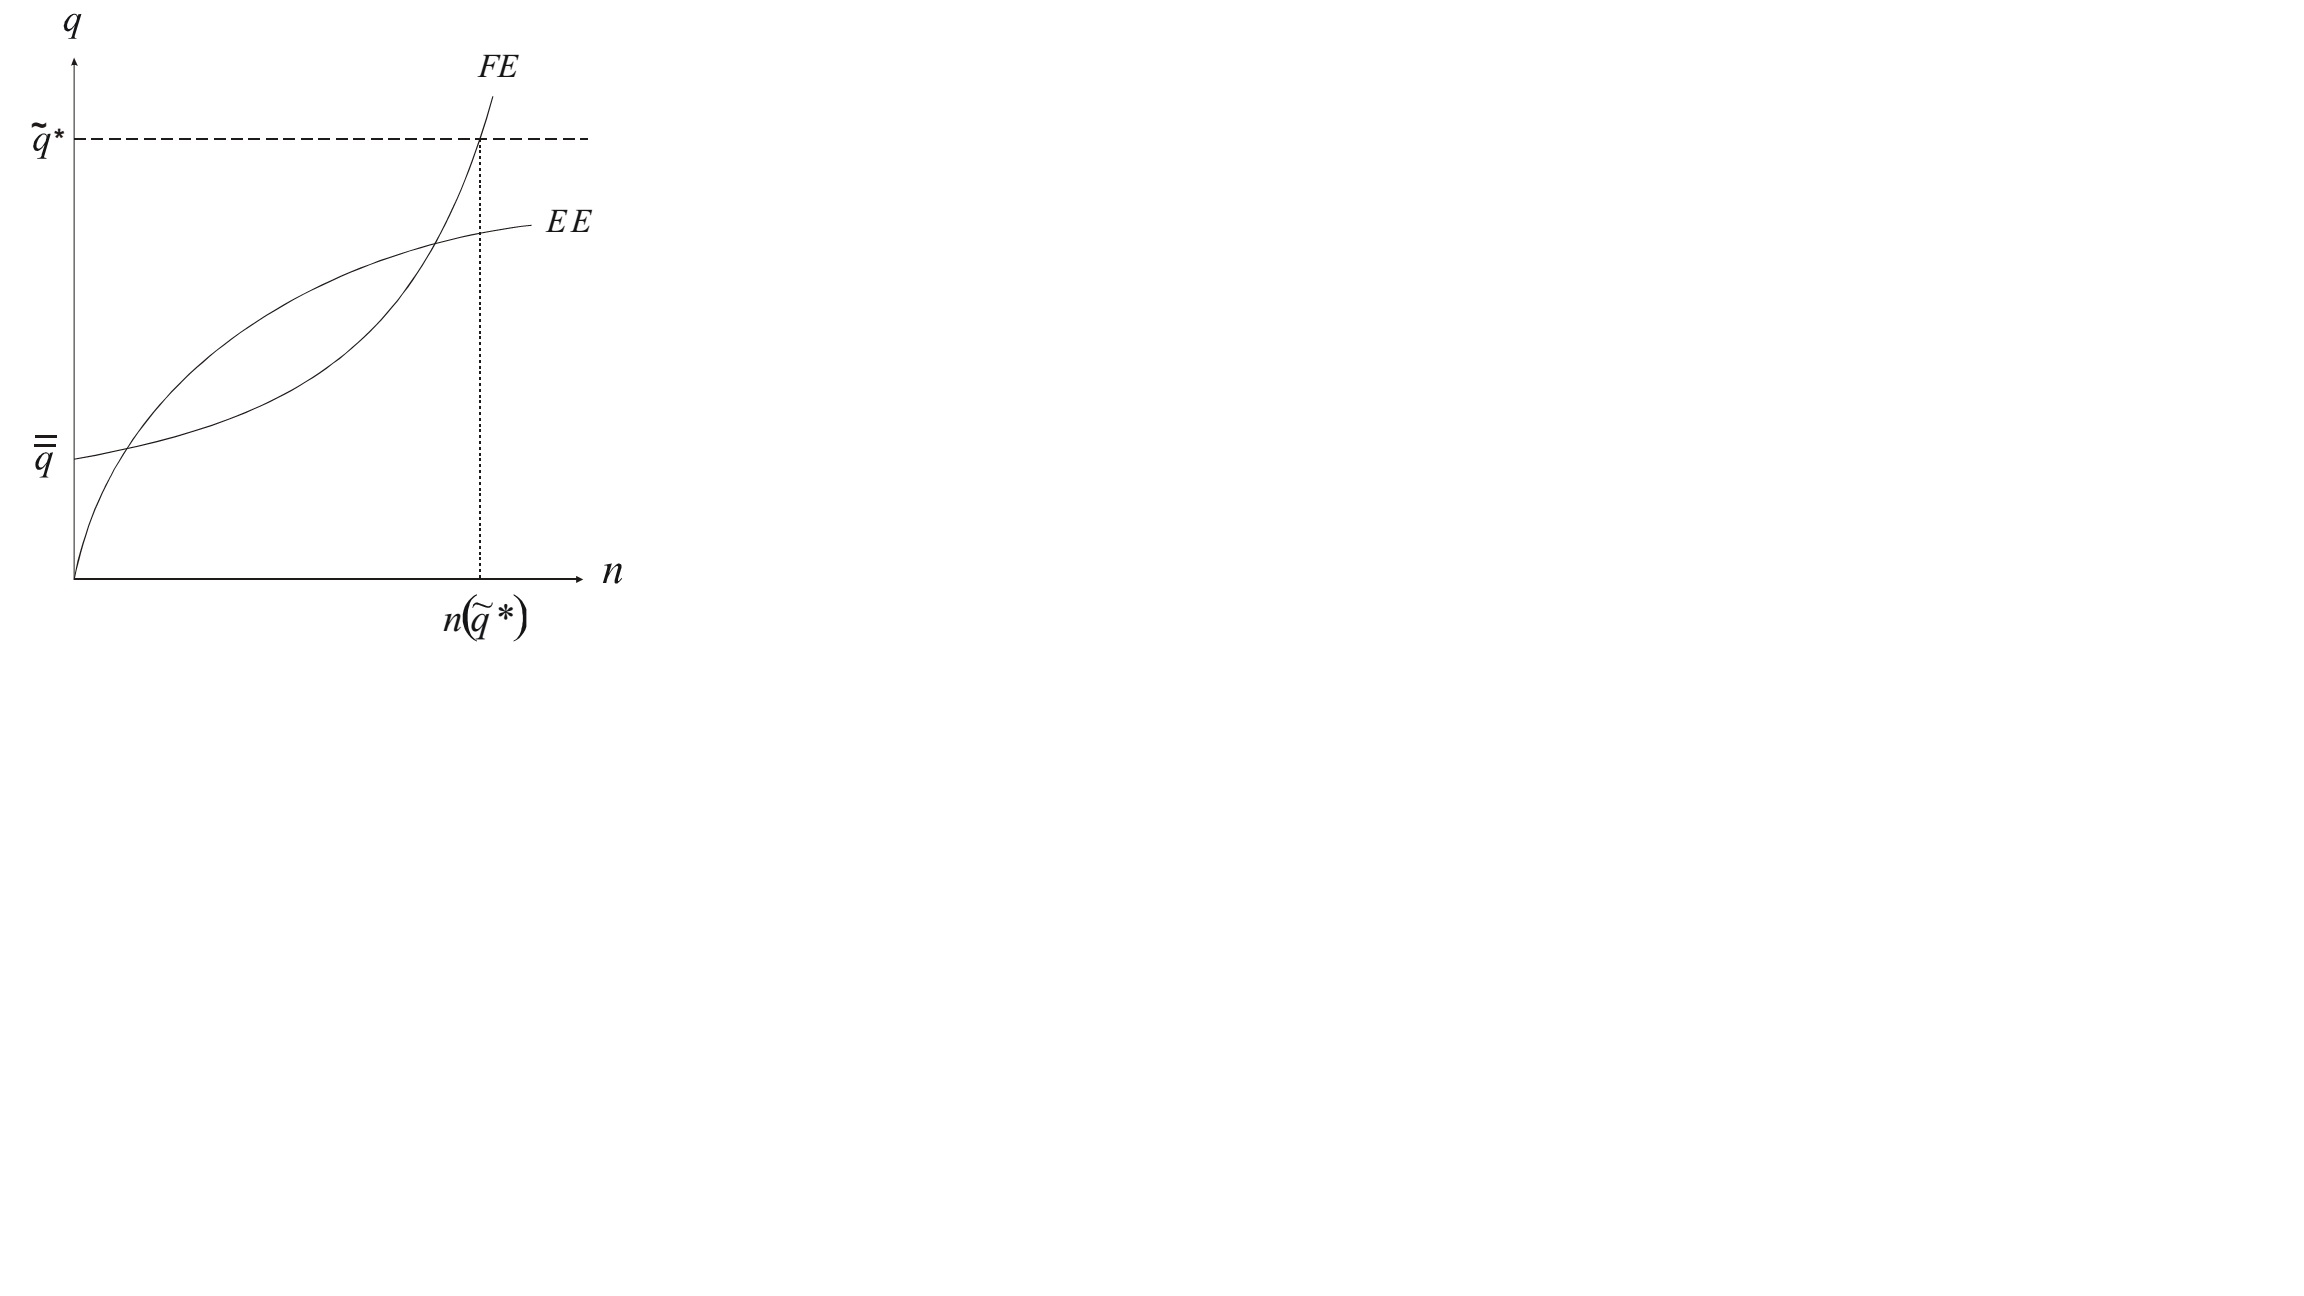
\includegraphics[scale=0.4]{1.jpg}
    \end{column}
\end{columns}

\end{frame}

\begin{frame}{Competitive Equilibrium}
    \begin{itemize}
        \item Suppose that there is a Walrasian auctioneer during the night and the numbers of buyers and sellers must be same in the market.
        \item While the market is competitive, buyers and sellers have to queue to randomly get in it.
        \item Money is still useful. (Why?)
    \end{itemize}
\end{frame}
\begin{frame}{Competitive Equilibrium}
    \begin{itemize}
        \item Taking the price as given, buyers and sellers solve the following problems:
        \begin{align*}
            \max_{q_{b}}&\left\{u(q^{b})+\beta_{n}W_{+1}^{b}(m_{b}-pq_{q})\right\}\\
            &\text{s.t. } pq_{b}\leq m_{b}\\
            \max_{q_{s}}&\left\{-c(q^{s})+\beta_{n}W_{+1}^{s}(m_{s}+pq_{q})\right\}
        \end{align*}
            \item Still, given $\gamma \geq \beta$, $m_{b} < m^{*}$. Thus, $q_{b} = m_{b}/p$
    \end{itemize}
\end{frame}

\begin{frame}{Competitive Equilibrium}
     \begin{itemize}
        \item F.O.C.
        \begin{align*}
            c'(q^{s}) = \beta_{n}\phi_{+1}p
         \end{align*}
         \item Take the derivative of $V^{b}(m_{b})$ and combine it with the F.O.C
        \begin{align*}
 \frac{u'(q)}{c'(q)} = \frac{\gamma-\beta}{\beta\alpha(n)}+1 
        \end{align*}
        \item Free entry condition
        \begin{align*}
            \frac{\alpha(n)}{n}\left[qc'(q)-c(q)\right] = k
        \end{align*}

        
    \end{itemize}  
\end{frame}

\begin{frame}{Competitive Equilibrium}
    \begin{itemize}
        \item Given $k<q^{*}c'(q^{*})-c(q^{*})$, we have an unique equilibrium iff $\gamma=\beta$, and multiple equilibrium iff  $\gamma\in(\beta,\bar{\gamma})$, for some $\bar{\gamma}$.
        \item When $\gamma=\beta$, $q^{*}$ can be achieved here since there is no holdup problem under competitive price.
        \item n is efficient iff $\frac{q^{*}c'(q^{*})-c(q^{*})}{ u(q^{*})-c(q^{*})} = \frac{n^{*} \alpha'(n^{*})}{\alpha(n^{*})} $ \item Generally, $n$ is inefficient and it may be higher or lower than $n^{*}$.
        \item Since at the better equilibrium $\partial n/\partial \gamma<0$, as long as $n>n^{*}$, we may improve the welfare by raising $\gamma$ at $\gamma=\beta$.
        \item search externalities: congestion effect versus thick effect
        
    \end{itemize}
\end{frame}

\begin{frame}{Competitive Search Equilibrium}
    \begin{itemize}
        \item Market makers open sub-markets during the night.
        \item Market makers can post different trade contracts $(q,d)$ and charge participants an entry fee.
        \item Based on rational expectations, agents face a trade-off between the probabilities of meeting and price.
        \item A seller's problem is:
        \begin{align*}
            W^{s}(m_{s}) = \phi m_{s} + \beta_{d} \underbrace{\max_{(q,d,n)}\left\{\frac{\alpha(n)}{n}\left[-c(q)+\beta_{n}W_{+1}^{s}(d)\right]\right\} }_{J_{s}}+\beta W_{+1}^{s}(0) 
        \end{align*}
    \end{itemize}
\end{frame}

\begin{frame}{Competitive Search Equilibrium}
    \begin{itemize}
               \item A buyer's problem is:
        \begin{align*}
            W^{b}(m_{b}) = \phi (m_{b}+T) + \max_{(q,d,n)}\left\{-\phi d+\beta_{d}\alpha(n)\left[u(q)-\beta_{n}\phi_{+1}d\right]\right\}\\+\beta W_{+1}^{b}(d) 
            \end{align*}
            \item Thus, we can rewrite the problem as
            \begin{align*}
            \max_{(q,d,n)} &\left\{\alpha(n)\left[u(q)-\beta_{n}\phi_{+1}d\right]-(\frac{\gamma-\beta}{\beta})\beta_{n}\phi_{+1}d\right\}\\
            &\text{s.t. }J_{s} = k
        \end{align*}
    \end{itemize}
\end{frame}

\begin{frame}{Competitive Search Equilibrium}
    \begin{itemize}
        \item Given $k<u(q^{*})-c(q^{*})$, the authors prove that there is a unique equilibrium if $\gamma \in (\beta,\bar{\gamma})$, for some $\gamma$.
        \item Market makers can play the role like a social planner to internalize the search externalities.
        \item  The holdup problem doesn't occur since buyers and sellers have to ``commit" to the contract before matching.
        \item Combining the above results, the equilibrium $(q,n) $ is efficient iff $\gamma=\beta$.
        
    \end{itemize}
\end{frame}
\section{Conclusion}
\begin{frame}{Conclusion}
    \begin{itemize}
        \item We analyzed the different market structures for monetary economies. 
        \item Market structures are important for the search friction and holdup problem.
        \item Depending on the different pricing mechanisms, the policy implication may change.
        \item We do not argue that one of the pricing mechanisms is correct, but provide a framework to clarify the role of friction in monetary economic.
    \end{itemize}
\end{frame}

\begin{frame}
    \centering
    \Large
    Thanks for your listening.
\end{frame}
\end{document}
